\section{Framework and Tools}
In this section, we gradually develop the framework. First, we decide what data source to use initially and describe how to use the data. Second, we present the method of choice to perform initial data filtering with. Third, we agree on which data storage and ingestion to use. Fourth, we provide a methodology to group the data with. Fifth, we decide how user interaction with the results will take place. Last, we select the visualisation tools to be used.
%In this section, we evaluate what data sources are useful. Additionally, we discuss several methods and tools that can be helpful in storing and ingesting data. Furthermore, we describe numerous methods to filter and classify textual data. Then, we elaborate on different methods to perform queries with. We conclude with an overview of the available visualisation tools that can be used for displaying the results of the analysis.

\subsection{Gathering the Data}
As explained in subsection \ref{sec:design-goals}, data sources should be plugable. An initial corpus of documents is needed to base the project, which we will decide on in this subsection. 

\subsubsection{Common Crawl} \label{sec:commoncrawl}
Common Crawl \cite{commoncrawl} is a freely accessible corpus of pages across the web, updated and released on a monthly basis. Many researchers have used the data for various purposes
\cite{smith2013dirt, muhleisen2012web, singh2012wikilinks}.
Since the project requires analysis on a very large set of documents, the corpus is a very suitable candidate for us to work with. \\

The data from Common Crawl comes in three formats\footnote{\url{https://gist.github.com/Smerity/e750f0ef0ab9aa366558}}: 
\begin{description}
\item[\textbf{WARC}] This is the default and most verbose format. It stores the HTTP-response, information about the request and meta-data on the crawl process itself. The content is stored as HTML-content.
\item[\textbf{WAT}] Files of this type contain meta-data, such as link addresses, about the WARC-records. This meta-data is computed for each of the three types of records (meta-data, request, and response). The textual content of the page is not present in this format.
\item[\textbf{WET}] This format only contains extracted plain text. No HTML-tags are present in this text. For our purposes, this is the most useful format.
\end{description}

Common Crawl stores these pages in the following way: each archive is split into many segments, with each segment representing a directory. Every directory contains a document listing file and a folder for each file format (WARC, WAT and WET), which in turn contains the compressed pages belonging to the segment. To be able to efficiently get a single page, Common Crawl indexes the segments to directly map URLs to document locations using an offset and length which can be found using the Common Crawl index\footnote{\url{http://index.commoncrawl.org}}. Since WAT- and WET-files can be generated from WARC-files, they only provide such indices for WARC-files. If no file index is provided with a data request, an aggregated compressed file of all files of the requested format is returned.

For extracting data from Common Crawl, many open-source libraries are available. Common Crawl's official website refers to \texttt{cdx-index-client}\footnote{\url{https://github.com/ikreymer/cdx-index-client}} as a command line interface to their data indices. It allows for, among others, specifying which data set to use, supports multiple output formats (plain text, gzip or JSON) and can run in parallel. Since this library only retrieves the file indices, we need another way to actually retrieve the pages pointed to. However, there is a problem with this: we are only interested in WET-files, but Common Crawl does not have WET-files indexed. We would therefore have to collect the WARC-files and convert them to WET-files ourselves, requiring us to parse HTML for every document we are interested in.

A simple query on the latest index using the online interface\footnote{\url{http://index.commoncrawl.org/CC-MAIN-2017-13-index?url=*.nl&output=json&showNumPages=true}} yields 1676 pages. Pages in this sense are listings of 15000 indices, so there are roughly 25 million entries in total. It is very important to note that searching for a top level domain like \texttt{.nl} only includes the first page of every matching domain. To get all pages, additional queries for each site with more than one page are to be performed.


\subsubsection{Other Data Sources}\label{sec:delpher}
Besides Common Crawl, there are a plethora of other sources that might contain valuable information. The most notable is the Dutch royal library, Delpher\footnote{\url{http://delpher.nl}}. It contains millions of Dutch digitalised newspapers, books and magazines from the fifteenth century up until about 1995. Because of this, it is a useful resource for historical research. Additionally, Statistics Netherlands\footnote{\url{https://www.cbs.nl/en-gb}} is the governmental organisation collecting statistical data about the Netherlands and comes with an API, making most of their data publicly accessible. The NOW Corpus\footnote{\url{http://corpus.byu.edu/now/}} collects newspaper and magazine articles through Google News and provides several tools to perform queries on this data. It can also be downloaded. 

Due to time and resource constraints, we have chosen to exclude these from the project. Of course, in future versions, other data sources could be included.



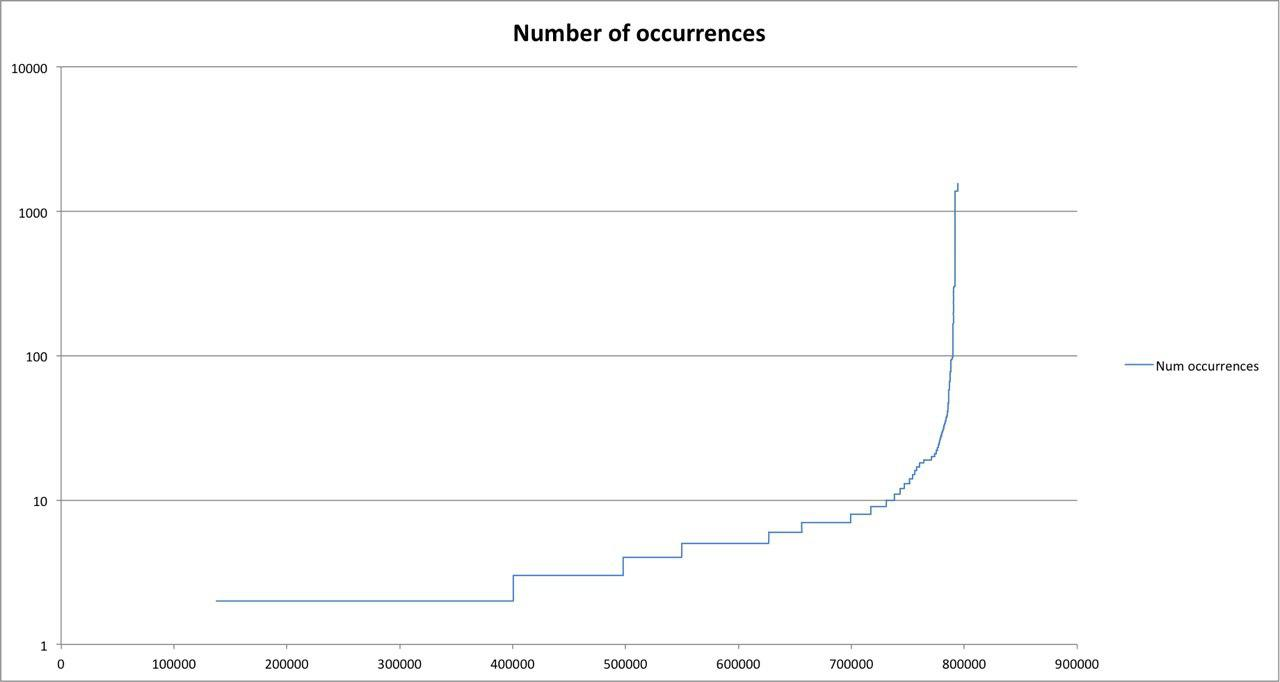
\includegraphics[width=\textwidth]{occurences_per_page}
% \todo{add info:}

% Piet Bep, [16.06.17 11:55]
% num 20
% 773665
% num 30
% 7510
% num 40
% 4020
% num 50
% 979

% Piet Bep, [16.06.17 11:55]
% bovenstaande is aantal documenten met minder dan 20 occurrences, tussen 20 en 30, tussen 30 en 40, en tussen 40 en 50
\subsection{Filtering Documents}
Because not all data from information sources such as Common Crawl is relevant to find relationships between cities, the data needs to be filtered. One way to do this, is to only select the data that mentions at least two different cities. Because the data is plain text, we need a way to scan through the text and determine if the text indeed has a co-occurrence of two different cities.
Making use of the comparative analysis of Rasool et al. \cite{rasool2012string}, we chose the Aho-Corasick algorithm \cite{Aho-Corasick}, which is a multi-pattern exact string matching algorithm and is the driver of widely used tools such as \texttt{grep} \cite{kernighan1984unix}. The algorithm creates a finite state machine, where strings to match are final states. Since we are looking for the co-occurrence of cities, using a multi-pattern string matching algorithm is preferred over a plain string matching algorithm. This is especially well illustrated by table \ref{tab:bm-matching} below. The benchmark was performed on a string of 1500 characters, with a million iterations. In the table, the average speed of matching is shown in seconds.

\begin{table}
\centering
\begin{tabular}{ |c|c| } 
    \hline
    multi-pattern matching & 0.000049831339 \\
    plain string matching & 0 \\
    \hline
\end{tabular}
\caption{Benchmark of multi-string vs. plain string matching}
\label{tab:bm-matching}
\end{table}

Using the Aho-Corasick algorithm, a predefined list of cities can be matched against the text of a web page or document. If at least two cities from the list appear in the text, we mark it as a useful document.

The decision to use the Aho-Corasick algorithm is strengthened by the fact that a well documented and stable Python library exists, which implements the aforementioned algorithm. This library is called \texttt{pyahocorasick}\footnote{\url{https://pypi.python.org/pypi/pyahocorasick/}} and is a fast and memory efficient implementation of the Aho-Corasick algorithm.

We make a selection of documents without storing the documents first, because storing all documents is not feasible due to storage constraints. For the .nl web pages only would need about 250 GB of storage and to store all available documents around 250 TB of storage would be needed. As we do not have access to a fast and large data storage platform, we will not store everything first and then delete documents that were filtered out. However, to test if finding and storing relationships between cities is fast enough when the documents are actually stored on disk a random selection of 1 million documents will be downloaded. Processing the already stored documents could finish within one day\footnote{On a virtual server with 8GB RAM, 4 CPUs and 100GB of HDD storage.} whereas downloading all documents will most certainly take multiple days.

\subsection{Storing and Ingesting the Data}
In this section we will discuss which data storage solution we are going to use and why. We will compare a few options and select one that we think is the best choice. We will then briefly explain how it works and how we plan to use it.

\subsubsection{Graph database, search engine or traditional database}
To store the relevant data we can can choose from 3 categories that could best suit our needs, these categories are Graph Databases, Search Engines or traditional databases. Because we want to visualise the network of cities as a graph and are interested in relations between cities we want to use a Graph Database. A Search Engine is less useful for this project because as a user you don't want to search through the documents but you want to be able to explore the relations that can be extracted from the data. A Graph Database is a better choice compared to traditional relational databases because relations are the most important in the graph data model where this is not true for traditional relational databases. Therefore, we will be using a Graph Database.

\subsubsection{Comparing Graph Databases}
Now that we've established that we will be using a Graph Database, we need to choose which Graph Database we're going to use. To do this we made a table in which we compare aspects that are important to us of the available Graph Databases.\\


\noindent\begin{threeparttable}
\begin{tabular}{@{} *6l @{}}    \toprule
\emph{name} & \emph{Open-source} & \emph{Scalable} & \emph{Python support} & \emph{Free} & \emph{Built-in Visualisation}\\  \\\midrule
AllegroGraph    & \XSolidBrush  & \Checkmark  & \Checkmark  & \XSolidBrush\tnote{a} & \XSolidBrush\tnote{b} \\ 
ArangoDB  & \Checkmark & \Checkmark & \Checkmark & \Checkmark & \Checkmark\\ 
Neo4j  & \Checkmark & \Checkmark & \Checkmark & \Checkmark\tnote{c} & \Checkmark\\ 
OrientDB  & \Checkmark & \Checkmark & \Checkmark & \Checkmark & \Checkmark\\ 
Teradata Aster & \XSolidBrush & \Checkmark & \Checkmark & \XSolidBrush & \XSolidBrush\tnote{d}\\ 
Titan  & \Checkmark & \Checkmark & \XSolidBrush & \Checkmark & \XSolidBrush\tnote{e}\\\bottomrule
 \hline
\end{tabular}
\begin{tablenotes}
\item[a] Only free up to 5 million triples
\item[b] With separate tool called Gruff: \url{https://allegrograph.com/gruff2/}
\item[c] Non-commercial use
\item[d] Using a separate tool Aster AppCenter
\item[e] Using a separate tool 
\end{tablenotes}
\end{threeparttable}\\

From this table we can see that 3 of these graph databases are viable candidates, these 3 candidates are ArangoDB, Neo4j and OrientDB. We chose to use Neo4j out of these three because of two reasons. Firstly because we have experience with Neo4j, which means we have to spend less time getting to know the graph database and it's functions and language. Secondly because is by far the most popular graph database \footnote{\url{https://db-engines.com/en/ranking/graph+dbms}}. Because Neo4j is the most popular graph database the support community is bigger compared to other graph databases and there are plenty of examples and answers available online. Therefore, we will be using the Neo4j graph database.

\subsubsection{Neo4j}
Neo4j is a highly scalable native graph database that leverages data relationships as first-class entities \cite{neo4j}, enabling enterprises of any size to connect their data and use the relationships to improve their businesses. It is the single highly scalable, fast and ACID compliant \todo (see section \ref{sec:elastic-downsides} for a short explanation) graph database available. Additionally, it is free to use for non-commercial use. To illustrate how scalable Neo4j is, consider that very large companies such as ebay, Cisco, Walmart, HP and LinkedIn\footnote{\url{https://neo4j.com/customers/}} use it in their mission-critical systems. Holzschuher and Peinl compared the performance of Neo4j to the more classic and commonly used NoSQL databases and found out that the more natural representation of relationships resulted in significant performance increase gains~\cite{holzschuher2013performance}.

There are some specific aspects of Neo4j that make it a very suitable candidate for this application. These are:

\begin{description}
\item[properties] Any entity in the Neo4j graph can be given properties (key-value pairs) containing information about the entity. Properties are primarily meant to provide additional information and are less suitable to be queried on. As an example, a city can have a number of inhabitants and districts attached to it as a property.
\item[labels] Nodes can be tagged with a label, describing their roles in the network. These annotations are especially useful to filter the data set on one or more categories. For example, a city can be labelled as "capital" to be able to distinguish between regular and capital cities.
\item[relations] Nodes can be connected using relationships. These are always directed, typed and named and can have properties. Using these properties, one can control how the graph is traversed. For example, if a path (relationship) is to be avoided unless absolutely necessary, the relation can be given a high cost. To give importance to some relationship, one could also assign a strength score to it. Since relationships are handled efficiently by Neo4j, nodes can have any number of relationships linked to it without compromising performance. For our purpose, a relation could comprise the strength of the relationship between two cities (nodes).
\end{description}

The Neo4j model can be depicted as shown in figure \ref{fig:neo4j}. It consists of nodes, relationships (edges), properties (within the nodes) and labels (rectangular blocks above the nodes).

\begin{figure}
\centering
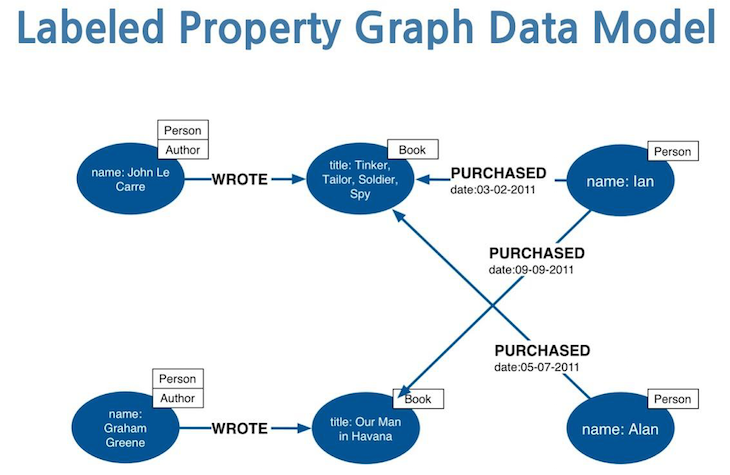
\includegraphics[width=0.75\textwidth]{neo4j}
\caption{The Neo4j model}
\label{fig:neo4j}
\end{figure}

Besides the aforementioned useful properties of Neo4j, we can put the graph to good use for visualising the global urban network. By adding a location property to a city, we can directly map nodes and relations to a geographical map. Most importantly, we can store indices of text files that mention the city as properties of nodes. That way, we are able to generate a subset of files that we can analyse for calculating the strength of the relationship between the nodes.









% --------------------------------------------Maybe useful in future----------------------------------------------------
\begin{comment}
\subsubsection{Elasticsearch}
Elasticsearch is an open-source search engine which centrally stores your data \cite{Elasticsearch}. It is a fast and scalable solution that was designed with big data search in mind. According to Kononenko et al. \cite{Kononenko2014} Elasticsearch has some significant advantages in comparison with traditional relational databases. Two of these advantages are scalability and performance. 

\paragraph{Scalability} According to Elasticsearch \cite{Elasticsearch} their product has no problem with scaling horizontally. It automatically manages indices and queries distributed across a cluster. This is an important feature as it is likely that the amount of data that our solution will use and process will increase and we do not want to keep upgrading the server that contains database, which would be vertical scalability. {\color{red} FIXME: Referentie naar dat we alleen NL doen nu? En daarom scalability nogal belangrijk is}

\paragraph{Performance}
Because Elasticsearch was designed to handle documents and perform full-text search it not surprising it performs well doing this. As we're going to be using the same kind of input data we expect Elasticsearch as the most choice. Kononenko et al. found that while scalability and schema-free documents are common for NoSQL systems, the combination of all three (scalability, agility, and performance) in one system is what makes Elasticsearch stand out from other systems. Following this, we conclude Elasticsearch would be a good choice as a data storage and search platform for our {\color{red} FIXME: solution|product|project.. (We moeten even kiezen welke we aanhouden zodat we dat overal hetzelfde doen}.\\

\paragraph{Downsides} \label{sec:elastic-downsides}
A downside of Elasticsearch is that it does not have any form of security out of the box. This means that everyone with the server address could access the data. This is not a problem for CommonCrawl data, as this was already available online anyway. However, when using for example Delpher or other sources you need a license this becomes a problem. Next to that, it would also be possible for anyone to meddle with the data in Elasticsearch making the data unreliable. Elasticsearch provides a Security package for which you unfortunately need a paid license. However, to secure Elasticsearch while making it available for users we could use a plugin such as Search Guard\footnote{\url{http://floragunn.com/searchguard/}} or use a special proxy as proposed by Kononenko et al. \cite{Kononenko2014}.

Another downside of Elasticsearch is that transactions involving multiple documents\footnote{\url{https://www.elastic.co/guide/en/elasticsearch/guide/current/concurrency-solutions.html}} are not ACIDic. Where ACID stands for the four properties atomicity, consistency, isolation and durability regarding transactions in database systems \cite{haerder1983principles}. This means that we need to keep concurrency problems in mind and will probably need to enable some locking to prevent these concurrency problems when performing transactions on multiple documents. 



\subsubsection{Hadoop}
Because we are designing a \maybe{application} that will use and parse a lot of data, it will be useful to use distributed computing. Although we only use the .nl data \maybe{Totale grootte van data noemen?} from CommonCrawl for this \todo{project} (see section \ref{sec:commoncrawl}) we could still benefit from distributed computing, especially with the future of the \maybe{application} in mind. 
Therefore we want to use Apache Hadoop, which is a framework that allows for the distributed processing of large data sets across clusters of computers using simple programming models \cite{Hadoop}. With this open source software we could distribute the computations from a single server across many more devices, thereby speeding up the process. 

\end{comment}
\subsection{Grouping the Data}
After the indexes of websites are stored in Neo4J we want to group each website according to subject: for example economy, politics and migration. There are two methods that can be taken for this: clustering and classifying. Clustering means grouping without first defining what groups (or classes) should be used while classifying does need classes do be defined first. \\
A standard approach for grouping is to use only the text from the websites and removing all other data. The big advantage is that it costs much less storage. Information from images may be lost however. Since we have to go over millions of pages, storage is a big issue for us therefor we choose this approach. \\
Text based classification/Cauterization itself can be split on structured and unstructured text. Text is structured when sentences are used, meaning grammar is used. In the case of structured texts a word may say something about the next word in the sentence, therefor other techniques can be used (for example n-grams) then in case of unstructured texts.Because the text from websites can be structured as well as unstructured, we will most likely use unstructured approaches. One way to do this is by using machine learning.

\subsubsection{Pre-processing}
Before we can use the unstructured text we need to pre-process it. There are three steps to this. 
\begin{enumerate}
\item Tokenization. \\ splitting up the text into words and other symbols called tokens.
\item Removing stop words. \\ Removing all common words (the, a, an etc) and symbols ('.', ',', '!', etc). 
\item Stemming. \\ Reducing derived words to their stem (e.g. fishing -> fish).
\end{enumerate}
The programs Snowball \cite{snowball_dutch} and NLKT \cite{nlkt_stemming} (which uses the snowball version) have a dutch implementation for this, although it might need to be improved a bit.

\subsubsection{Clustering}
One method of grouping websites is clustering. For clustering text documents the standard approach is using k-means clustering, which uses the bag of words model. Scikit-Learn \cite{scikit-learn} has a library for this. In this library you can specify what feature extractors are used (TfidfVectorizer for tf-idf, a method for determining weights of words, and HashingVectorizer which hashes the words). Furthermore this library automaticly places the documents in batches if it would become too big to do it in one time. Initially we will test this method, however as we don't know whether we will get valid results we will keep the other method (classifying) in mind.

\subsubsection{Classifying}
Classifying is done in two steps: choosing the classes and actual classifying. Classes can be chosen manually, however, you can also apply certain techniques to automatise results. The advantage of this that you will get unbiased results, the disadvantage is that it takes more time to make these results and it may also cause classes to be chosen which the user can't use, for example when using Google Trends  \cite{googleTrends}  results as "AFC Ajax", "Aeroflot" and "Eric Dane" may be found. The same problem occurs when searching for sub-classes.\\

\textbf{Defining classes}\\
One problem we need to solve is the problem of choosing classes. This can be done in several ways. The easiest way is to define these ourselves, however we may get better results if we used some algorithm. When using algorithms we may also decide if we want to consistently use the same classes for each pair of cities, or define the classes per pair depending on the importance. For example if Rotterdam and Vlissingen have a huge trade of fish, "fish" we be an important class of the relation between Rotterdam and Vlissingen. However if Leiden does nothing with fish, the class will be absent for the relation Rotterdam-Leiden or Vlissingen-Leiden. One way to do this is to look at the websites for each relation and apply the 'bag of words' model to check which words occur most frequently (after stemming and the removal of stop words). To make sure we don't get similar results (for example the relations 'fish' and 'fishmarket') we could remove all websites containing 'fish' and then applying the same model again. Our plan is to first find some general classes (e.g. economy) from all websites. And then make subclasses (e.g. fish) for each pair. The general classes are used to compare between relations of different cities.\\

\textbf{Machine Learning for classification of unstructured text}\\
Text based machine learning for unstructured texts is done using the 'bag of words'. This model counts how often each word is used. There are 3 libraries available which contain most steps needed. There is scikit-learn \cite{scikit-learn} and TensorFlow \cite{tensorFlow} for Python and Weka \cite{weka} for Java. Since we write our program in python, and TensorFlow is only about neural networks, we choose to use scikit-learn.
The machine learning works in 4 steps:
\begin{enumerate}
    \item \textbf{Creating a feature extractor} \\
    To prepare the features for the machine learning algorithm. We need to give each feature/token a numeric id. Count each of these tokens. And we need to normalise the tokens. For this scikit-learn provides algorithms.
    
    \item \textbf{Manually labelling} \\
    For each of the classes (e.g. business, tourism, art etc) we select a few websites we know fit to that class. Here occurs the problem of defining classes which will be expanded on later. From these websites all the words will be extracted and their occurrence will be counted. Possibly some normalisation functions are applied to get better values. We call these values the weight for each word for each class. From this we create a two dimensional array with in the rows each of the websites and in the columns all different words and one extra for the class. We fill the fields with the weights or a zero if the words don't occur.
    
    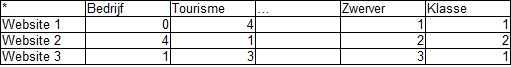
\includegraphics{classTable}
    
    \item \textbf{Generating a classifier} \\
    The array is fed to a learning algorithms. This will generate a classifier. There are a multitude of classifiers importable from Scikit-learn and TensorFlow. For choosing the classifier we make use of the Microsoft Azure Machine Learning Test Sheet \cite{MLCheatSheet}. Several factors should be taken into account when choosing an algorithm. These are:
    \begin{enumerate}
        \item Accuracy - How well the algorithm separates the websites.
        \item Training Time - How long it takes to train the algorithm.
        \item Linearity - Linear regression assumes data trends follow a straight line. This is trade-off between accuracy and speed.
        \item Number of Parameters - Adjustable parameters increase the flexibility of the algorithms. This is a trade-off between training time and accuracy.
        \item Number of Features - A large number of features can make some algorithms unfeasibly long. Especially text data (what we are using!) has a large number features. Support Vector Machines are especially well suited in this case.
        \item Special Cases - Some learning algorithms make particular assumptions about the data or the results.
    \end{enumerate}
    
    For textual data especially support vector machines are recommended, so it is most likely we will choose that machine learning algorithm. Depending on whether we have time we might do some tests before making our decision however.
    
    \item \textbf{Entering new examples} \\
    When a new (unlabelled) example (website) comes - extract the features and feed it to your classifier - it will tell you what it thinks it is (and usually - what is the probability the classifier is correct). Afterwards the classifier can be updated to include new features extracted from the example. This updating probably needs to be done a couple of times because the first few times not all features (possible words in the dutch dictionary) will be included. It is important to choose the same amount of websites for each class.
\end{enumerate}

\subsubsection{Conclusion}
Our approach will be to first transform the data into the bag of words model using tokenizing, stemming and the removal of stop words. Afterwards we will try to group the websites in 3 tries. First we try to cluster all the websites into groups. We will then whether these clusters are actually viable clusters and whether they can be labelled into useful categories. If this is not the case we will instead try classification. To define classes we will try to look at the most common words. Then removing all associated websites and repeating this until multiple words are chosen as categories. If even this does not work we will define our own categories.
After all websites are initially clustered or classified we will use the same method for the websites for a pair of cities. We will try to automatically assign the found relations to one of the main categories as well (e.g. fish to economy, train to travel etc). \\
After all websites are classified or clustered and possibly sub-classified or sub-clustered we can use that data to show the strengths of the connections between cities by counting for each class how many websites there are that contain information about both cities. \\
An earlier problem we encountered was differentiating between the cities Utrecht and Groningen and the provinces Utrecht and Groningen. We might be able to use machine learning as well to check if a website is talking about the province or the city, however it could very well be that this does not significantly improve our data.

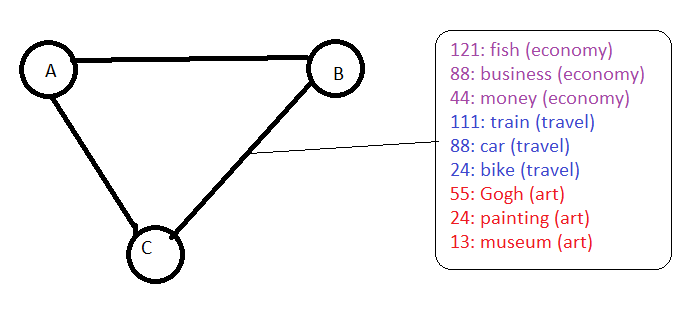
\includegraphics{classificatie}
\subsection{Interacting with the Data}

For the application to be a success the processed data should be easily available to the end user. The data should be easy to query and should be presented in an accessible way.
We researched several options to offer the end user this experience.

\subsubsection{Query language}

The first option was to develop an easy to use/learn query language specific to our domain (intercity relations). For this we designed a simple query language with the following syntax.

\begin{center}
\begin{tabular}{ |c|c| } 
 \hline
 ! & Logic NOT operation \\
 \&\& & Logic AND operation \\ 
 $\|$ & Logic OR operation \\ 
 $( A \&\& B )$ & Grouping of clauses \\
 $A > R > B$ & Relation R between cities A and B \\
 \hline
\end{tabular}
\end{center}

Below, in figure \ref{fig:ql-example}, an example is shown that queries the "Shopping" relation between Rotterdam and Amsterdam and the same relation between Rotterdam and Den Haag.

\begin{figure}[ht]
\centering
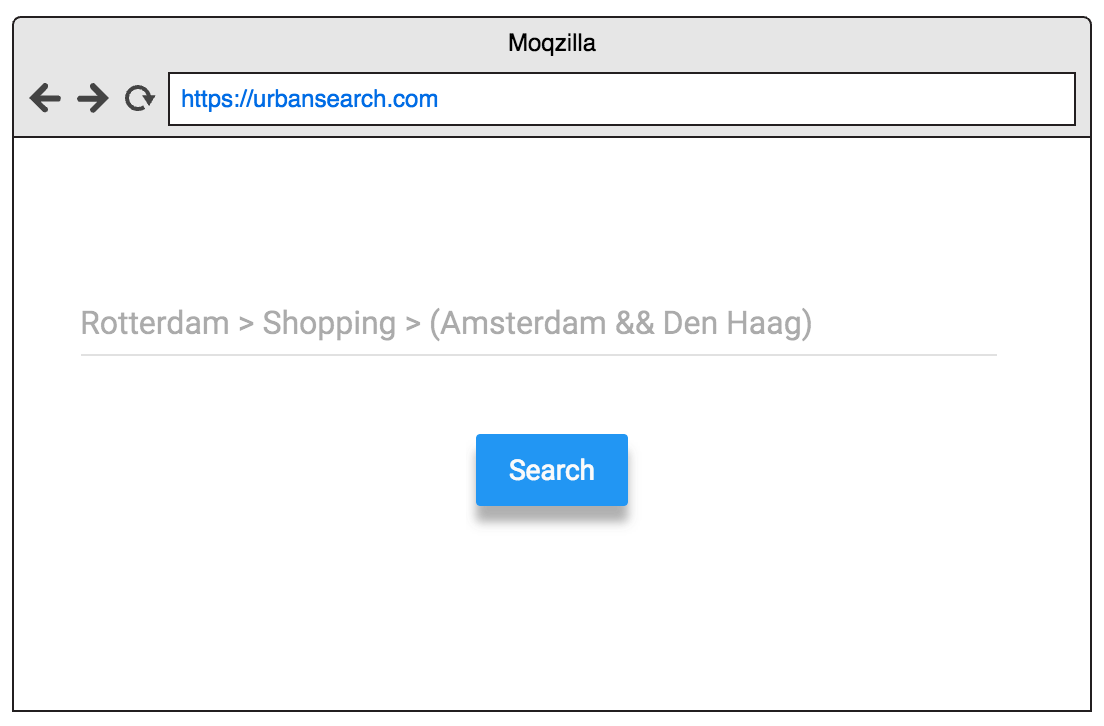
\includegraphics[width=0.75\textwidth]{ql-example}
\caption{Example interface for the query language}
\label{fig:ql-example}
\end{figure}

\subsubsection{Query composer interface}

Another option was to offer the end user a "query composition interface". This interface would have the same possibilities as the former mentioned query language, but should be more intuitive to use for new users. An example of the interface is given in figure \ref{fig:qi-example}.

\begin{figure}[ht]
\centering
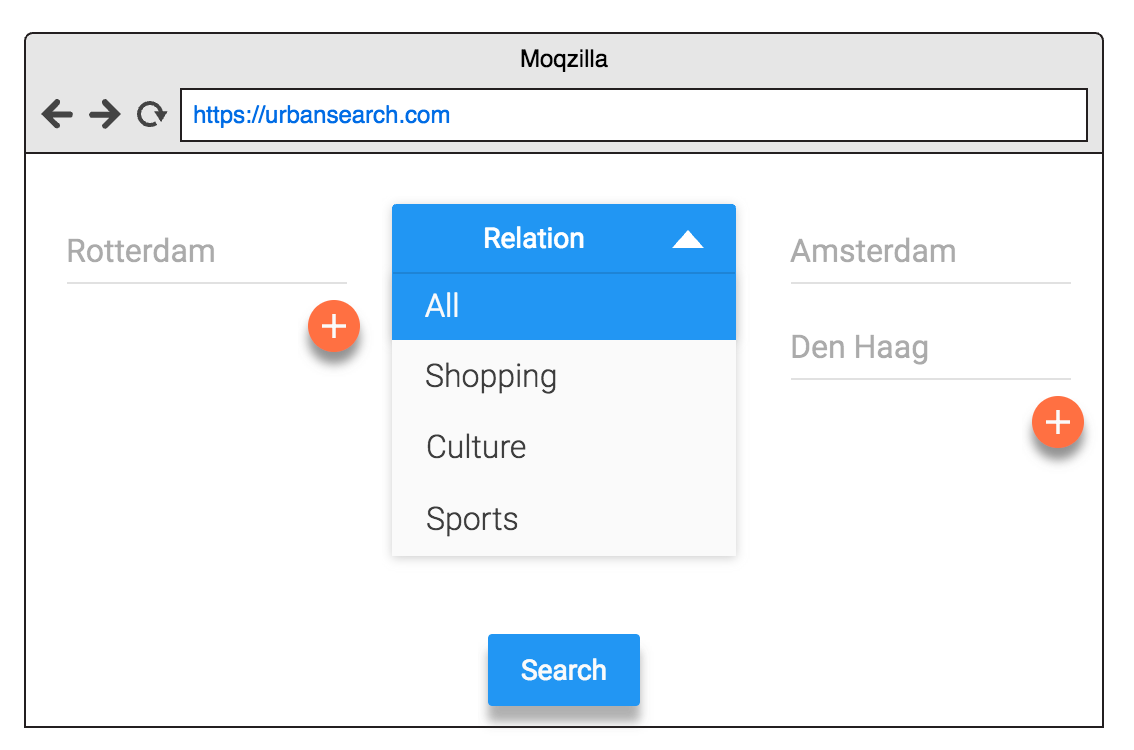
\includegraphics[width=0.75\textwidth]{qi-example}
\caption{Example of a query composer interface}
\label{fig:qi-example}
\end{figure}

\subsubsection{Interactive search}

The last option we investigated was an interactive approach to querying data. This means that the user interacts with a map containing relations and cities. A very simple example is given in figure \ref{fig:ii-example}.


\begin{figure}[ht]
\centering
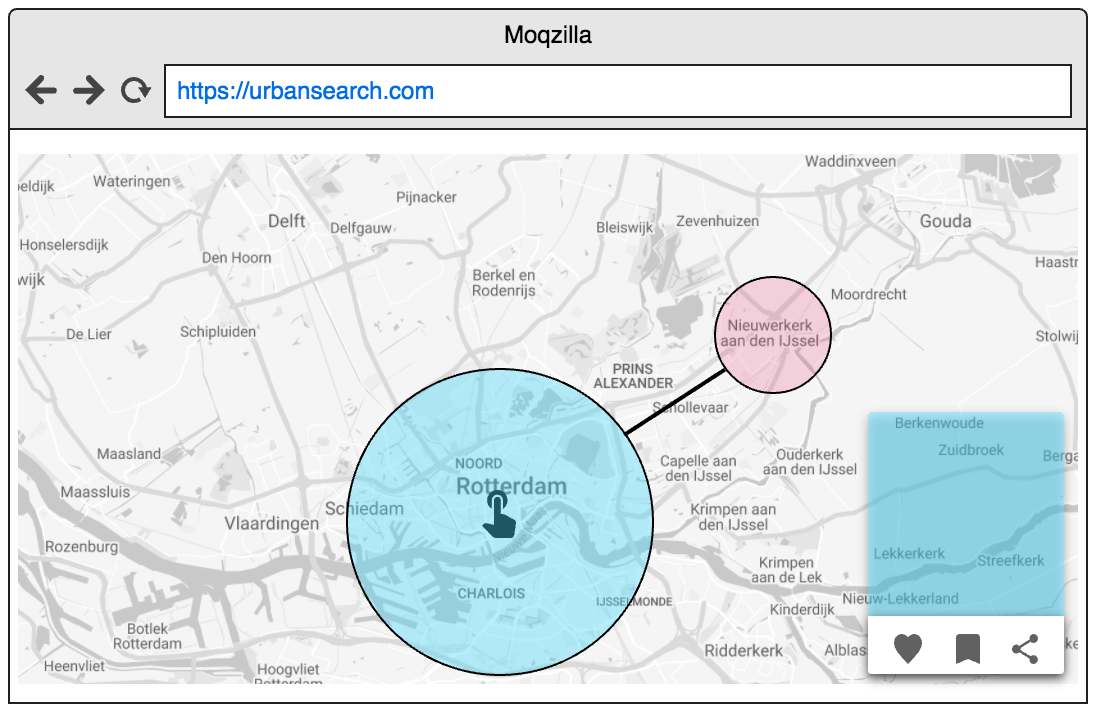
\includegraphics[width=0.75\textwidth]{ii-example}
\caption{Example of an interactive map}
\label{fig:ii-example}
\end{figure}

In this setup the user can click on cities and relations on the map which then triggers a query on the Neo4j back-end. The results can be visualised on the map (eg. showing information about the selected city).

\subsubsection{Conclusion}

Together with the client we decided that the best option was to go with the interactive map. This would lead to easy access to the data by the client and would fit better with the flow of use the client envisioned prior to the project. 
Also from the point of view of the researcher using the application, it fits a lot better in his/her work flow. The application is used to analyse and visualise relations between cities, if this can be done directly on the map it speeds up the users use of the system, since it is faster to select cities and relations on the fly. This helps make the application more intuitive since the user is probably more familiar with a map than with a new query language.
The creation of complex queries is also made a lot easier. The user doesn't have to write or compose a complex query in advance but can do it directly on the map. So getting a visual representation of several cities, interconnected with multiple relations, doesn't mean writing or composing a very long query but clicking/selecting cities and relations on the map.
Interaction directly with the map also reduces the need to go to a separate page to enter/compose a query. This speeds up the use of the system by reducing page loads and it interrupts the work flow of the user less.
A final advantage of using an interactive map over raw queries/query composition is that we don't have users entering invalid queries, this leads to less frustration using the system.
\subsection{Visualising the Data}

This section focuses on the visual representation of the processed data. Our goals are to present the data and the things we learned during the processing of the data in a way that is easy to comprehend for users and can help ease the interpretation of the data.
To reach these goals we focused on the clients needs and desires. We discussed the preferences off the client and drew up a global plan, which we present below.

\subsubsection{Representing the data visually}

Since we are dealing with strongly related data, which is comprised off cities and the relations between cities, it was a natural choice to represent the data as a graph.
The choice was made, together with the client, to show the nodes and relations on a map. This was done because people are used to cities being visualised on a map and we think this will increase the ability of users to interpret the information in a productive manner.

\subsubsection{Maps}

We investigated two technologies we could use for the map on which we will display our data. The first one is Google Maps (GM). GM can be used freely and offers a lot of customisation options. The API is well defined and some of the group members worked with GM before. The second option we investigated was Leaflet. Leaflet is an open-source javascript library which provides responsive maps. It also has an well defined API and a lot of plugins.
Both libraries are well suited for our needs. 
We decided to go with GM, because of the experience of the group members with using GM. Also we feel that there are more resources available on GM, which would help us if we get stuck with an issue.

\subsubsection{Map clutter}

One of the challenges of visualising networks, as stated in \cite{468391}, is the risk of so called map clutter. This means the network is displayed as an incomprehensible set of lines and nodes.
Several methods to prevent this are given in \cite{468391}. We will adopt some of these methods in our application. The methods and use of these methods in our application are presented next.
Users should be able to select what information they want to display. This will be adopted in our application by allowing the user to (de)select cities and relations, which then will be shown/hidden. The use of different sizes for nodes and edges or other attributes that are displayed can convey extra information to the user. We will use this to represent sizes of cities (population) and strengths of relations.
The use of colour is another method which is presented in \cite{468391}. We will use colours to represent different types of relations and we will use intensity/opacity to represent the strengths of these different types of relations.